\chapter{Module assembly}

There several ways to assemble the module. Usually high-precision sensors for high energy physics are constructed manually with a help of mechanical jig.

\section{Manual assembly with mechanical jig}

One option for module assembly is manual assembly with a custom-built mechanical jig (prototype is shown on Figure \ref{fig:mechanical_jig}) \cite{Automated_assembly_slides}.

\begin{figure}[ht]\centering
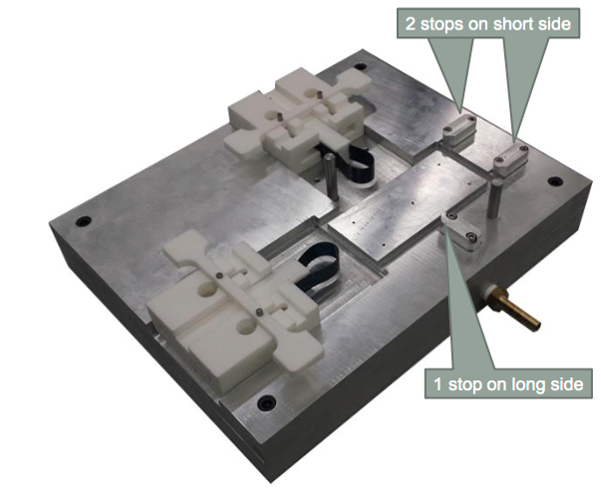
\includegraphics[width=0.7\linewidth]{Data/Module_assembly/Mechanical_jig.png}
\caption{Prototype of the mechanical jig for module assembly.}
\label{fig:mechanical_jig}
\end{figure}

With such method of assembly all parts are placed in the jig and glued together manually. To provide required accuracy mechanical jig has 3 reference stops: one along longer side of the module and two along shorter side. From opposite to reference stops sides the module is gently pushed by springs towards reference stops. Together they provide enough precise positioning of the module's components before and during gluing. 

However such method of module assembly has a number of disadvantages. It is relatively slow and does not scale well for high number of modules to assemble. In addition, such mechanical system has poor repeatability and has no options to control the process. Moreover, it needs very precise machining technologies (several microns precision) to manufacture this mechanical jig, as well as calibration of reference stops positions. Finally, this mechanical system need maximum manual handling and highly depends on human operating it. This fact means that even though in theory system can provide required quality of the assembled modules, there will be always more or less several percentage of modules assembled out of required quality only because of a human mistake.

\section{Automated assembly}

\section{Automated assembly steps}

[Perhaps I should put this section later...?]
Steps [list]:
1) Spacers to platform
2) Glue upper sensor to spacers
3) Rotate 90 degrees
4) Remove spacer+upper sensor
5) Put baseplate on the assembly platform
6) Glue bottom sensor (bare module) to the baseplate
7) Glue Upper sandwich to the bottom one.


\section{Assembly platform}




\subsection{Requirements for assembly platform}



\subsection{Design}



\section{Fast adhesive}

